
%----------------------------------------------------------------------------------------
%	Lecture 5
%----------------------------------------------------------------------------------------

\chapter{Autonomous Equations} 

\bigbreak

\section{Introduction}

Autonomous Equations are of the form : 
$$ \diff{y}{t} = f(y) $$
That is, there is no independent variable on the right hand side.
We can solve this equation by separation of varibales.
But here we will learn how to extract information out of this equation without solving it.

\section{Direction Fields, Isoclines and Integral Curves}

Here, we can see that any horizontal line $y = y_0$ is an Isoclines of this equation because $f(y)$ is constant on such a line.
And the slope of all the line elements on this line is $f(y_0)$.

\begin{figure}[ht!]
    \centering
    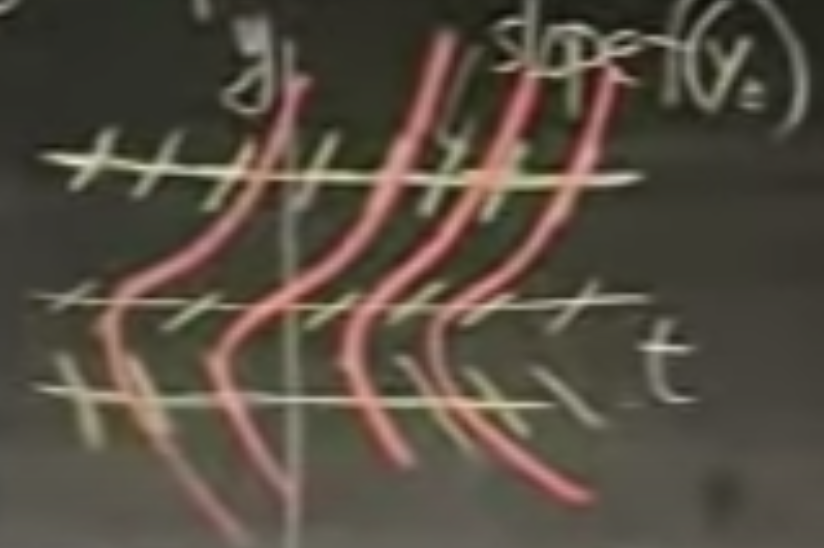
\includegraphics[scale=0.5]{./images/lecture_5_figure_1.png}
    \caption{Direction Fields, Isoclines and Integral Curves of an Autonomous Equation}
\end{figure}

Here we can see that all the integral curves are the same and they only differ in the constant term.
Thus, you can get all the curves by just drawing a single curve and moving it horizontally.

\section{Critical Points}

A Critical Point of the equation is a point where $f(y) = 0$.
Now if $f(y) = 0$ is zero at $y = y_0$ then this line is a solution to the equation.
Because the slope of the line is zero and the right hand side is also zero by definition.


The importance of this solution is that it serves as a barrier.
Since two integral curves can never cross each other.

So if we have two solutions to $f(y) = 0$ being $y = y_0$ and $y = y_1$ then the integral curves in between those can never esacpe the region between these lines.
Also for any integral curve between these lines, we must be able to move the curve horizontally to get another integral curve which does not intersect any other integral curve.
That limits their behaviour very much.

The method to find the integral curves is to first find the Critical Points.
Then we plot the graph of $f(y)$ to find where is it positive / negative / zero.
This is important because we want to find the slope at a point to see whether it is increasing or decreasing.

{\bf Example : } Let's say $y$ is the account balance in the bank and $r$ is the constant interest rate.
Let $w$ is the rate of withdrawl.
So $$ \diff{y}{t} = ry - w $$

Here, we have a critical point at $y = \frac{w}{r}$.
So there is a solution $y = \frac{w}{r}$.
Now if $y > \frac{w}{r}$ then $f(y) > 0$ and if $y < \frac{w}{r}$ then $f(y) < 0$.
So the solution is increasing when $f(y) > 0$ and the solution is decreasing $f(y) < 0$.

So if the initial value is above the line $y = \frac{w}{r}$ then it increases forever.
And if the initial value is below the line $y = \frac{w}{r}$ then it decreases forever.

Now, we only need to draw two solution because all other solutions can be found by moving these two solutions horizontally.

\subsection{Logistic Equation}

This eqaution models the population behaviour $y(t)$ over time.
$$ \diff{y}{t} = ky $$
where $k$ is the net growth rate.

If $k$ is constant then it is called simple growth.

Logistic Growth is when $k$ decreases as the population increases.
The simplest decreases function of $y$ is $k = a - by$.
Our new equation is 
$$ \diff{y}{t} = ay - by^2 $$

The critical points are $y = 0$ and $y = \frac{a}{b}$.
So we have two constant solutions.

\begin{figure}[ht!]
    \centering
    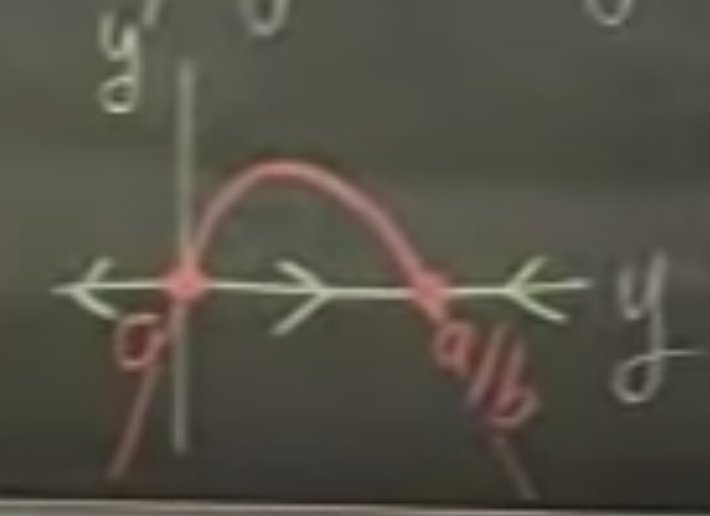
\includegraphics[scale=0.6]{./images/lecture_5_figure_2.png}
    \caption{Plot of $f(y)$ against $y$}
\end{figure}

Now for the inbetween, $f(y) = ay - by^2$ is a downward opening parabola with roots at $0$ and $\frac{a}{b}$.
So it is positive if $0 < y < \frac{a}{b}$ and negative everywhere else.

So if we start in between the constant solution then it will always be increasing but it will never cross the constant line solution.

\begin{figure}[ht!]
    \centering
    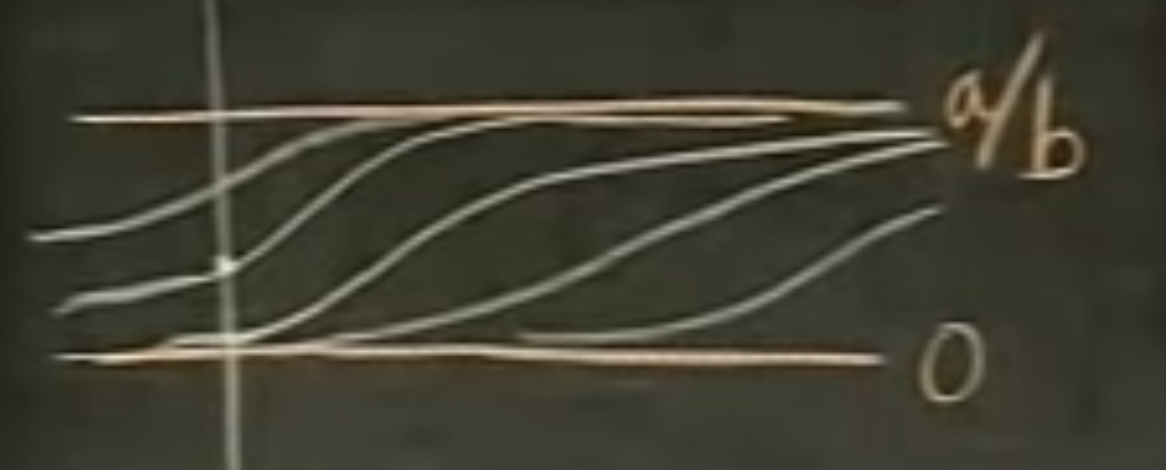
\includegraphics[scale=0.5]{./images/lecture_5_figure_3.png}
    \caption{Integral Curves Between $y = 0$ and $y = \frac{a}{b}$}
\end{figure}

If we start above $y = \frac{a}{b}$ then the curve will be forever decreasing without ever touching the line $y = \frac{a}{b}$.

If we start below $y = 0$ then the curve will be forever decreasing.

Thus, we can see that the solution $y = \frac{a}{b}$ is attractive, that is, every other solution approches this forever.
While $y = 0$ is replusive, that is, every other solution goes away from it.

Thus, $y = \frac{a}{b}$ is a stable solution and $y = 0$ is an unstable solution.
If all curve approach a point on one side and go away from it on the other side then the solution is called semi-stable solution.
\pagebreak
\subsection{Logistic Equation With Harvesting}

Here we assume that the harvesting is done at the rate $h$. 
So our equation is 
$$ \diff{y}{t} = ay - by^2 - h $$

Here, we can analyze this by plotting the graph with $h = 0$ and as we increase $h$, the graph goes lower and lower.
And the critical points come closer together.

\begin{figure}[ht!]
    \centering
    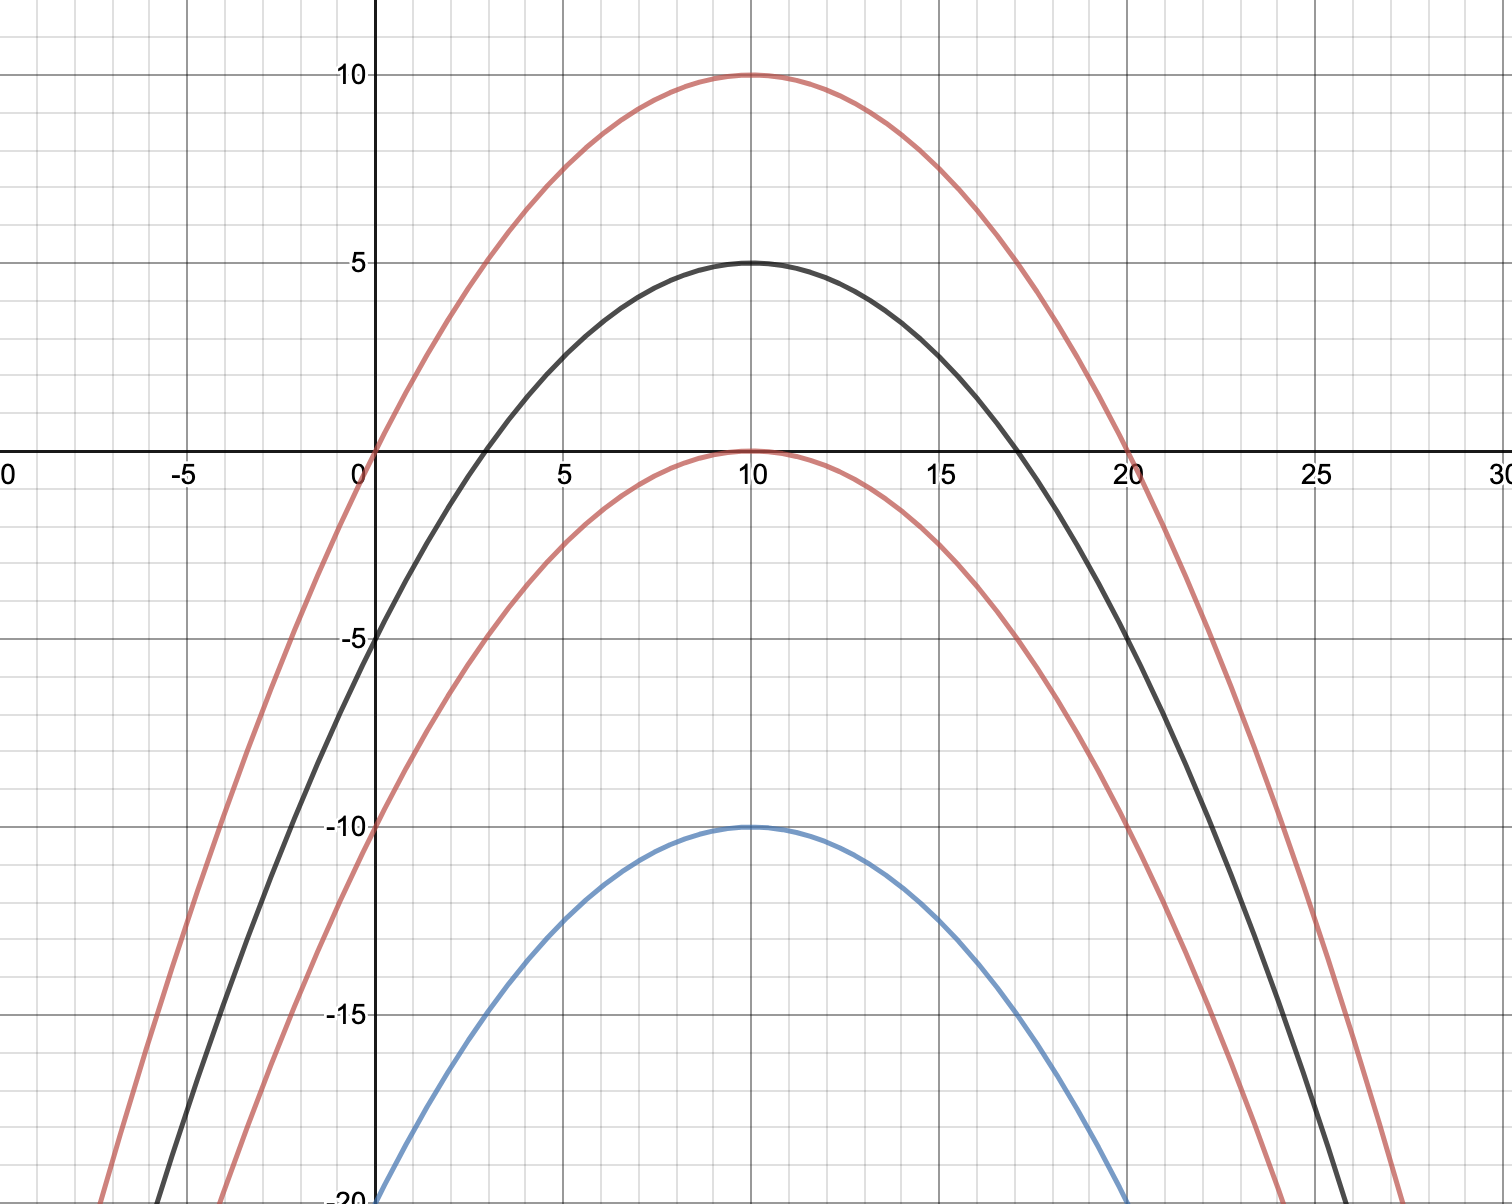
\includegraphics[scale=0.3]{./images/lecture_5_figure_4.png}
    \caption{Plot of $f(y)$ with different values of $h$}
\end{figure}

In the graph above, we can see that as we increase $h$ the critical points come closer and closer and at one point there is just one critical point.
The value of $h$ where there is only one critical is called $h_m$.
For any higher value of $h$ there are no critical points.


Now for $h = h_m$, there is just one critical point. 
For the points above the critical point, the function is decreasing so it will approch the critical point.
For the points below the critical point, the function is decreasing so it will keep decreasing forever going away from the critical point.
So the solution at the critical point is called the semi-stable solution.

\begin{figure}[ht!]
    \centering
    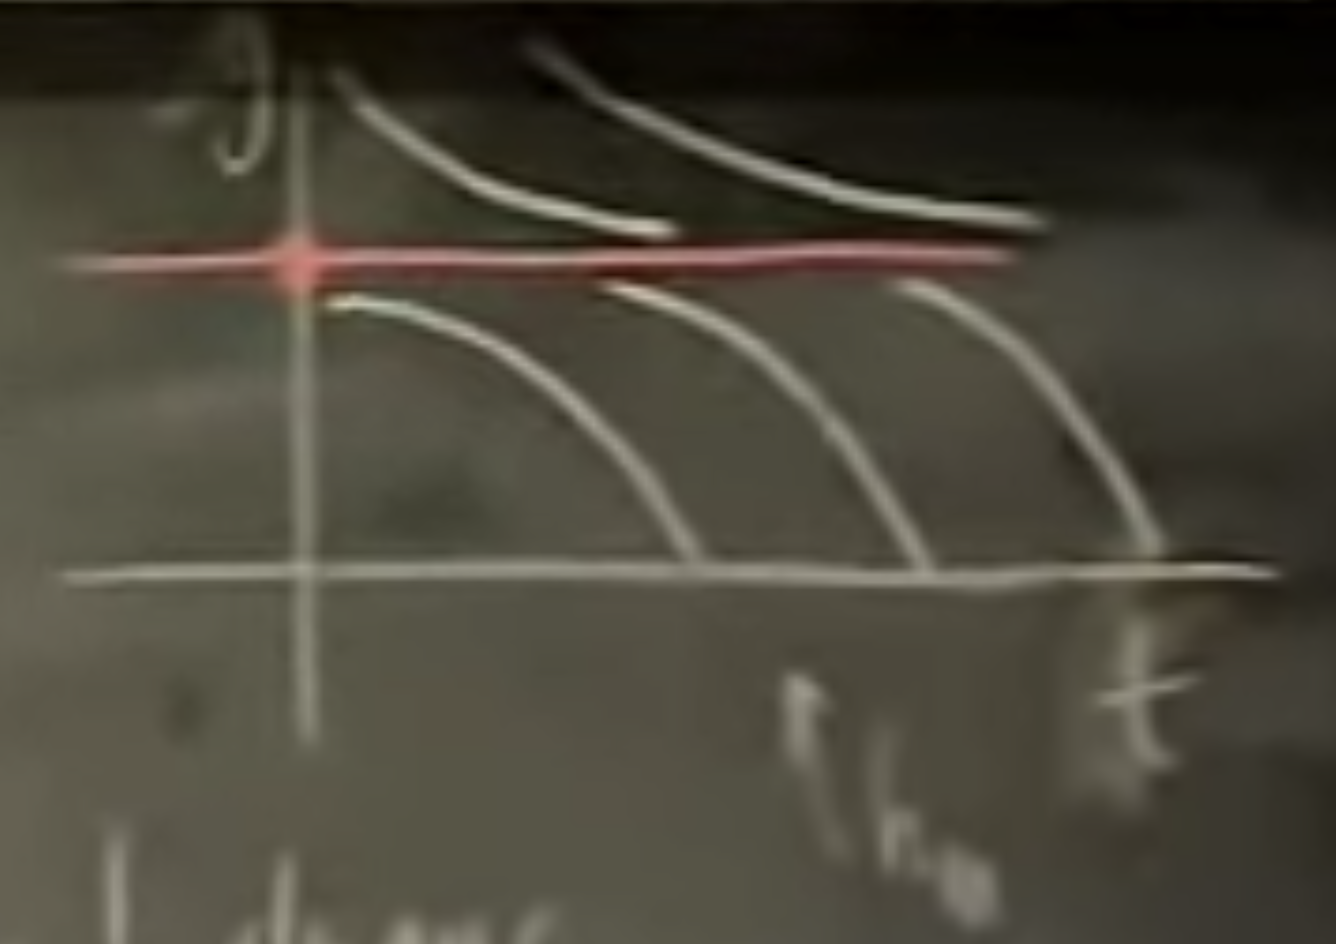
\includegraphics[scale=0.3]{./images/lecture_5_figure_5.png}
    \caption{Solutions of the Equation with $h = h_m$}
\end{figure}

If there are no critical points then the solution is always decreasing and goes to negative infinity.